\subsection{VLSI Integrators and Differentiators}

Now we're going to blend the observations we've just made about low pass and high pass filters with what we know of the transconductance amplifier to do some cool things. Let's refresh our mind as to what the transconductance amplifier is all about: 

\begin{itemize}
    \item $I_{out} \approx g_m(V_1 - V_2) \ \mathrm{with} \ g_m = \frac{I_b \kappa}{2 U_T}$
    \item $I_{out} = I_1 - I_2 = I_b\frac{e^{\frac{\kappa V_1}{U_T}} - e^{\frac{\kappa V_2}{U_T}}}{e^{\frac{\kappa V_1}{U_T}} + e^{\frac{\kappa V_2}{U_T}}} = I_b \mathrm{tanh}(\frac{\kappa (V_1 - V_2)}{2U_T})$
    \item $g_d = - \frac{\partial I_{out}}{\partial V_{out}} \approx \frac{I_b}{V_E}$
    \item $A = \frac{\partial{V_{out}}}{\partial{(V_1 - V_2)}} = \frac{\partial {V_{out}}}{\partial{I_{out}}} \frac{\partial {I_{out}}}{\partial{(V_1 - V_2)}} = \frac{g_m}{g_d} \approx \frac{\kappa V_E}{2U_T}$
\end{itemize}

\paragraph{What is the problem with the filters we've seen before?}
In VLSI technology, the time-constant of RC circuits implemented with passive elements cannot be changed once the chip has been fabricated. Both resistance and capacitance are fixed at design time by the geometries of the layout mask layers (this is the subject of NE2). By contrast, the transconductance amplifier has a transconductance that depends on its bias voltage
which can be set on the operating chip. Therefore, this device can be used to design an integrator circuit that has an \textbf{adjustable time-constant}: This follower integrator, which was first designed by Carver Mead in 1989, is shown in Figure \ref{fig:Follower_Integrator}. But before looking at the follower integrator, let's look at the unity gain follower, which will allow us to better understand the follower integrator. 

\subsubsection{Unity Gain Follower} 

SHOULD I INCLUDE THIS SECTION IN THE PREVIOUS CHAPTER? 

\begin{figure}[H]
    \centering
    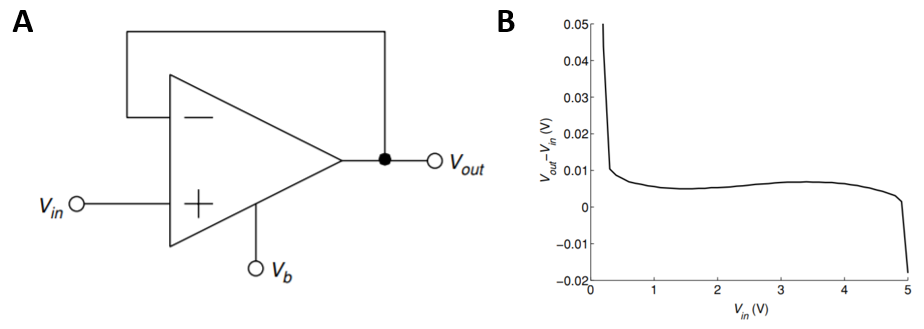
\includegraphics[width=0.9\linewidth]{../../Figures/Unity_Gain_Follower.PNG}
    \caption{A) Unity Gain Follower circuit. B) Deviation of output voltage from input voltage for simple unity-gain follower. Adapted from Textbook.}
    \label{fig:Unity_Gain_Follower}
\end{figure}

Most circuit applications use the transconductance amplifier as part of a negative-feedback loop (WHAT DOES THIS MEAN?). The negative feedback ensures that the amplifier stays within its operating range. The simplest negative feedback loop is obtained by short-circuiting the output terminal and the inverting input terminal, as shown in Fig. \ref{fig:Unity_Gain_Follower}.A. The transfer function of this circuit is given by:

\begin{equation}
    \frac{dV_{out}}{dV_{in}} = \frac{A}{A + 1} \approx 1
\end{equation}

Additionally, we should also define the input and output impedance: 

\begin{equation}
    \mathrm{Input \ Impedance: \ } Z_{in} = \frac{dV_{in}}{dV_{in}} \rightarrow \infty
\end{equation}
\begin{equation}
    \mathrm{Output \ Impedance: \ } Z_{out} = \frac{dV_{out}}{dV_{out}} = \frac{1}{g_d} \approx \frac{V_E}{I_b}
\end{equation}

Due to the large open-loop voltage gain A, the transfer function is almost unity with $V_{out} \approx V_{in}$. The circuit configuration is therefore called \textit{unity-gain follower}. It is used as an impedance converter (also called a buffer) and it converts a high input impedance (because the Transconductance amplifier draws no current) into a lower output impedance. In contrast to the source follower presented in the simple circuit chapter, which is also used as an impedance converter, the unity-gain follower does not introduce a large voltage offset. The measured deviation of the output signal from the input signal, $V_{out} - V_{in}$, as a function of the input voltage is shown in Figure \ref{fig:Unity_Gain_Follower}.B.


\subsubsection{Follower Integrator} 

\begin{figure}[H]
    \centering
    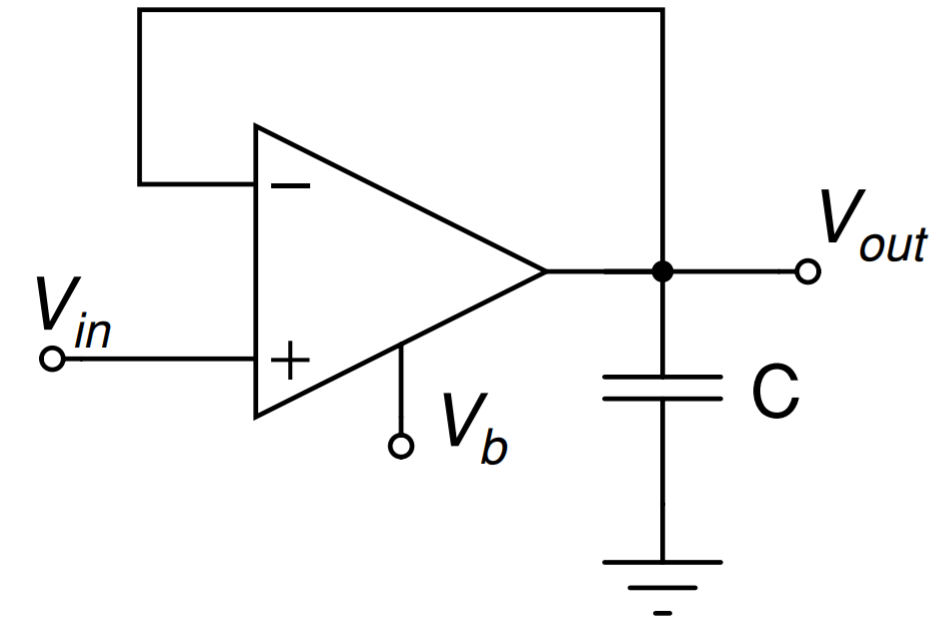
\includegraphics[width=0.5\linewidth]{../../Figures/Follower Integrator.PNG}
    \caption{Follower Integrator circuit. The bias voltage $V_b$ , which sets the transconductance amplifier’s bias current $I_b$, can be used to modify the integrator’s time-constant. Adapted from Lecture Notes. Adapted from textbook}
    \label{fig:Follower_Integrator}
\end{figure}

This circuit is built out of a unity gain follower and a capacitor connected to the follower's output node. The input voltage is applied to the $+$ terminal of the follower. If the circuit operates in subthreshold, we can apply Kirchoff's Current Law at the circuit's output node and reach the familiar looking equation: 

\begin{equation}
    C \frac{dV_{out}}{dt} = I_b \mathrm{tanh}(\frac{\kappa (V_{in} - V_{out}}{2 U_T})
\end{equation}

Yes, it should be familiar, because if we take conductance $G = \frac{\kappa I_b}{2 U_T}$ (assuming small signal regime which is why we get rid of the tanh function), we can get back to the equation: 

\begin{equation}
    \frac{C}{G} \frac{dV_{out}}{dt} + V_{out} = V_{in}
\end{equation}

Yes! This is exactly (as conductance is the inverse of resistance - $G = 1/R$) the differential equation that we derived for the low pass integrator filter in the previous section. Beautiful no? Instead of a resistor, we used our transconductance amplifier \textbf{for which we can modulate the conductance \footnote{By convention we speak of conductance for transconductance amplifier instead of resistance}}. So this circuit also has the following time constant: $\tau = C/G$. Note that the amplifier will operate in its linear range provided that V in does not change
too rapidly. Specially, we need $\frac{dV_{in}}{dt} < \frac{4U_t}{\tau}$. Under these conditions, the transfer function of our RC circuit and Follower Integrator are thus identical. 

\paragraph{What happens when $\frac{dV_{in}}{dt}$ is large?}
When the AC component of $V_{in}$ is large, the transconductance amplifier is no longer linear and the previous relation is invalid. For very large variations in V in, the output current of the transconductance amplifier saturates at $I_b$, which is the asymptote of the equation we first found ($C \frac{dV_{out}}{dt} = I_b \mathrm{tanh}(\frac{\kappa (V_{in} - V_{out}}{2 U_T})$.  In this condition, the transconductance amplifier
acts as a constant current source rather than as a linear conductance. While the difference $|V_{out} -   V{in}|$ is greater than 4UT , $V_{out}$ changes linearly with time. As the the difference enters the small signal regime, the amplifier begins to behave as a linear conductance and $V_{out}$ begins increasing (or decreasing) exponentially. 
Figure \ref{fig:Large_Signal_Follower_Integrator} shows the typical response of the follower-integrator circuit to
a large step voltage input. The rate of change of output voltage $\frac{dVout}{dt}$ in the region of constant slope, is defined as slew rate and is usually specified in units of $V / \microsec$. Slew rate is one measure of the performance limit of an operational amplifier, and is proportional to the maximum output current of the amplifier.


\begin{figure}[H]
    \centering
    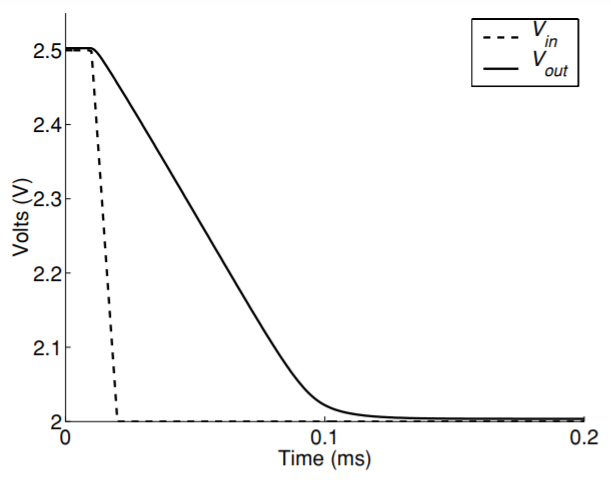
\includegraphics[width=0.5\linewidth]{../../Figures/Large_Signal_Follower_Integrator.PNG}
    \caption{Large signal behavior of a follower-integrator. Response of the circuit to a large negative step input
(dashed line). The output voltage $V_{out}$ decreases linearly for large difference $V_{out} -  V_{in}$ values and asymptotes exponentially for small differences. Adapted from textbook}
    \label{fig:Large_Signal_Follower_Integrator}
\end{figure}

\subsubsection{Delay Lines} 

\begin{figure}[H]
    \centering
    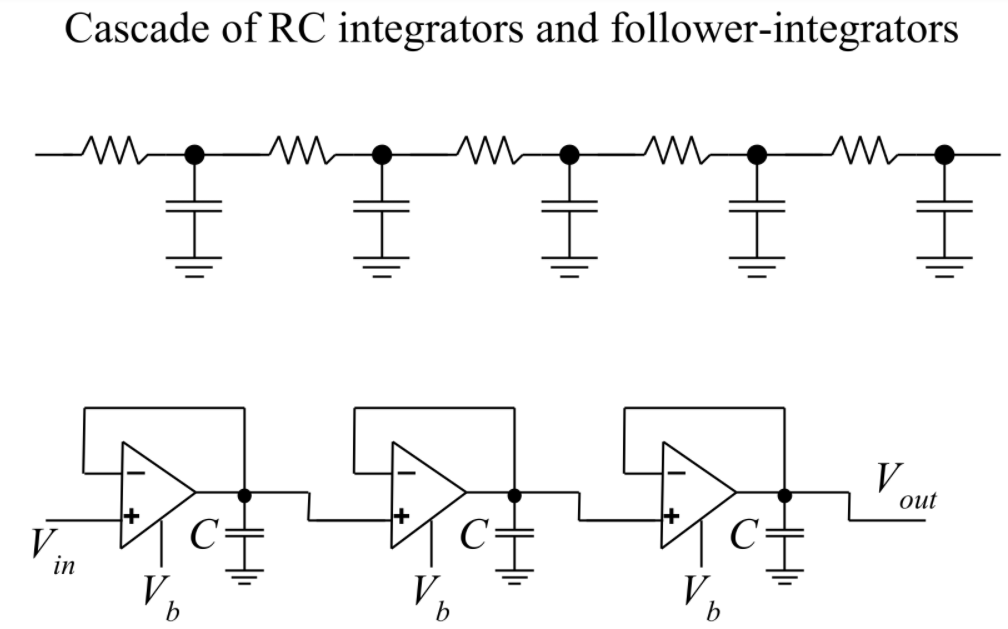
\includegraphics[width=0.65\linewidth]{../../Figures/Delay_Lines.PNG}
    \caption{Cascade of RC integrators (top) and follower integrators (down). Adapted from textbook}
    \label{fig:Delay_Lines}
\end{figure}

We can compose (connect) multiple instances of the R-C integrator circuit, or multiple instances of the follower-integrator circuit (see Figure \ref{fig:Delay_Lines}), in sequence to form a \textit{delay line}.
Each section in the delay line of \textbf{follower integrators} is modular (from a functional
point of view) and independent of the other sections. The current out of
the transconductance amplifier of one section can charge only the capacitor
connected to the output node: It is not affected by the other sections connected
to the output node. On the other hand, the sections of the R-C delay line of
are tightly coupled to one another. Current of one section flows into
both the capacitor of that section and the resistor of the next. Because the
characteristics of the single R-C circuit change when connected to other R-C
circuits (as in Fig. 9.3), the transfer function of the composition of R-C circuits
is not equal to the composition of individual transfer functions. Due to the modularity of the follower-integrator elements, the transfer function of the composition of follower-integrator circuits corresponds to the
composition of their individual transfer functions. For example, if the number of elements in the delay line in delay lines of follower integrators is $n$, we can simply use the transfer function of the regular RC integrator that was derived earlier and obtain: 

\begin{equation}
    \frac{V_{out}}{V_{in}} = \frac{1}{1 + \tau s}^n
\end{equation}


This is a very useful property, because it allows the frequency response
properties of the delay line to be evaluated analytically. Consider the case
where sinusoidal inputs are applied to the circuit of Follower integrator delay line. The delay line’s transfer function is:

\begin{equation}
    \frac{V_{out}}{V_{in}} = \frac{1}{1 + j\omega \cdot \tau}^n
\end{equation}

Exploiting the mathematical approximation that: 

\begin{equation}
    (1 + j \omega \cdot \tau) \approx (1 + \frac{1}{2}(\omega \tau)^2)e^{j \omega \tau} \mathrm{\ (for }\ \omega \tau \ll 1)
\end{equation}

We can write the transfer function explicitly in terms of magnitude and phase: 

\begin{equation}
    \frac{V_{out}}{V_{in}} \approx \frac{1}{1 + \frac{n}{2}(\omega \tau)^2)}e^{-j \omega n \tau}
\end{equation}

where the pre-exponential ratio is the magnitude and the exponential’s argument is the phase. From this equation, we can conclude that the magnitude of the output signal is attenuated by the factor $\frac{1}{2}(\omega \tau)^2$ as it crosses each section of the follower-integrator delay line, and the phase delay introduced by each section corresponds to $\omega \tau$ radians (equivalent to a time delay of $\tau$). This analysis is valid provided that each follower-integrator operates in its linear region. This is very useful to make better filters!

